\chapter{Using a CNN to solve the Problem}
\label{ch:solution}

As it is one of the most conventional approaches, we tried using a convolutional neural network built in \texttt{Tensorflow} \cite{tensorflow} to classify the images.
This, while not overly creative, seemed to be the safest approach to get good results. \\

Considering the amount of data available to us and that the dataset is indeed quite balanced, we chose accuracy as our metric.
We arbitrarily chose a set of parameters for the network, so that, once we had a relatively well-working model,
we could start optimising the hyperparameters. \\

As the input data were coloured images of size $256 \times 256$, we set the input shape to $(256, 256, 3)$.
The first model we used consisted of three convolutional layers with an ascending number of filters, 
each followed by a max-pooling layer before a flattened fully connected layer which in turn was followed by two dropout layers.
The exact structure can be seen in \autoref{fig:initial_model}. \\

\begin{figure}[H]
    \centering
    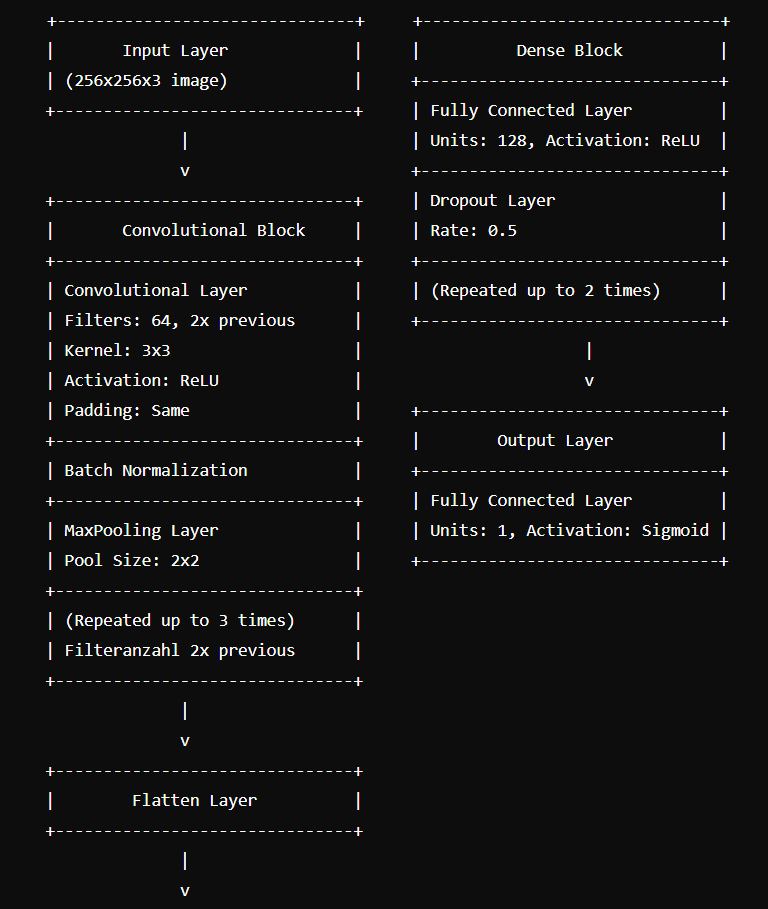
\includegraphics[width=0.5\textwidth]{images/initial_model.png}
    \caption{Structure of the initial model.}
    \label{fig:initial_model}
\end{figure}

While we considered whether a model with three layers was too powerful for the task at hand, we still wanted to test it out.
The increasing number of filters was chosen in order to allow the network to learn more complex features deeper into the model,
with the max-pooling layers picking out the most prominent features.
From the start, we tried avoiding overfitting as much as possible, thus the dropout layers.
The dropout we chose was in the region of around $50 \,\%$, as it seemed inefficient to throw away even more weights and insufficient to choose a lower dropout. \\

After each layer, we normalised the data using batch normalisation, hoping this would cut down on the rather substantial training time.
We used the ReLU activation function for the convolutional layers and the adam optimiser function for the output layer.
Again, these are the most common choices, with the adam optimiser drastically cutting down on training time, 
while the activation function was later used as a part of the hyperparameter optimisation. \\

And while is not yet time to talk about the results in depth, this did in fact not exactly produce the results we hoped it would.
Even though the accuracy was quite high at around $95 \,\%$, a closer look at the loss and accuracy curves showed that the model was greatly unstable
with jumps of over $20 \,\%$ in accuracy between epochs.


\section{Hyperparameter Optimisation}
\label{sec:results}

We still decided to perform a simple grid search, hoping that the instability arose from simply a poor choice of parameters.
The parameters we chose to optimise were the number of convolutional layers as well as the \texttt{max\_filters} within them, the dropout rate, the number of dense nodes
and the activation function.
Changing the learning rate did not seem necessary as, at the time, we used an adaptive learning rate in our model. 
Shown in \autoref{tab:gridparameters} are the different parameter values used in the grid search, while \autoref{fig:hyperparameter_optimisation_1} 
shows an excerpt of the $15$ best combinations. \\

\begin{table}[H]
    \centering
    \begin{tabular}{ll}
        \toprule
        \textbf{Hyperparameter} & \textbf{Chosen Values} \\
        \midrule
        Number of convolutional layers               & {$2, 3$}\\
        Maximum number of filters                    & {$32, 64, 128$}\\
        Dropout rate                                 & {$0.4, 0.5$}\\
        Number of nodes in dense layers              & {$128, 256, 512$}\\
        Activation function for convolutional layers & {LeakyReLU, ReLU}\\
        \bottomrule
    \end{tabular}
    \caption{Chosen Hyperparameters for Model Optimization}
    \label{tab:hyperparameters}
\end{table}

While this might not seem like a great amount of variation, this still provided $71$ different combinations and took multiple days to compute.



\begin{figure}
    \centering
    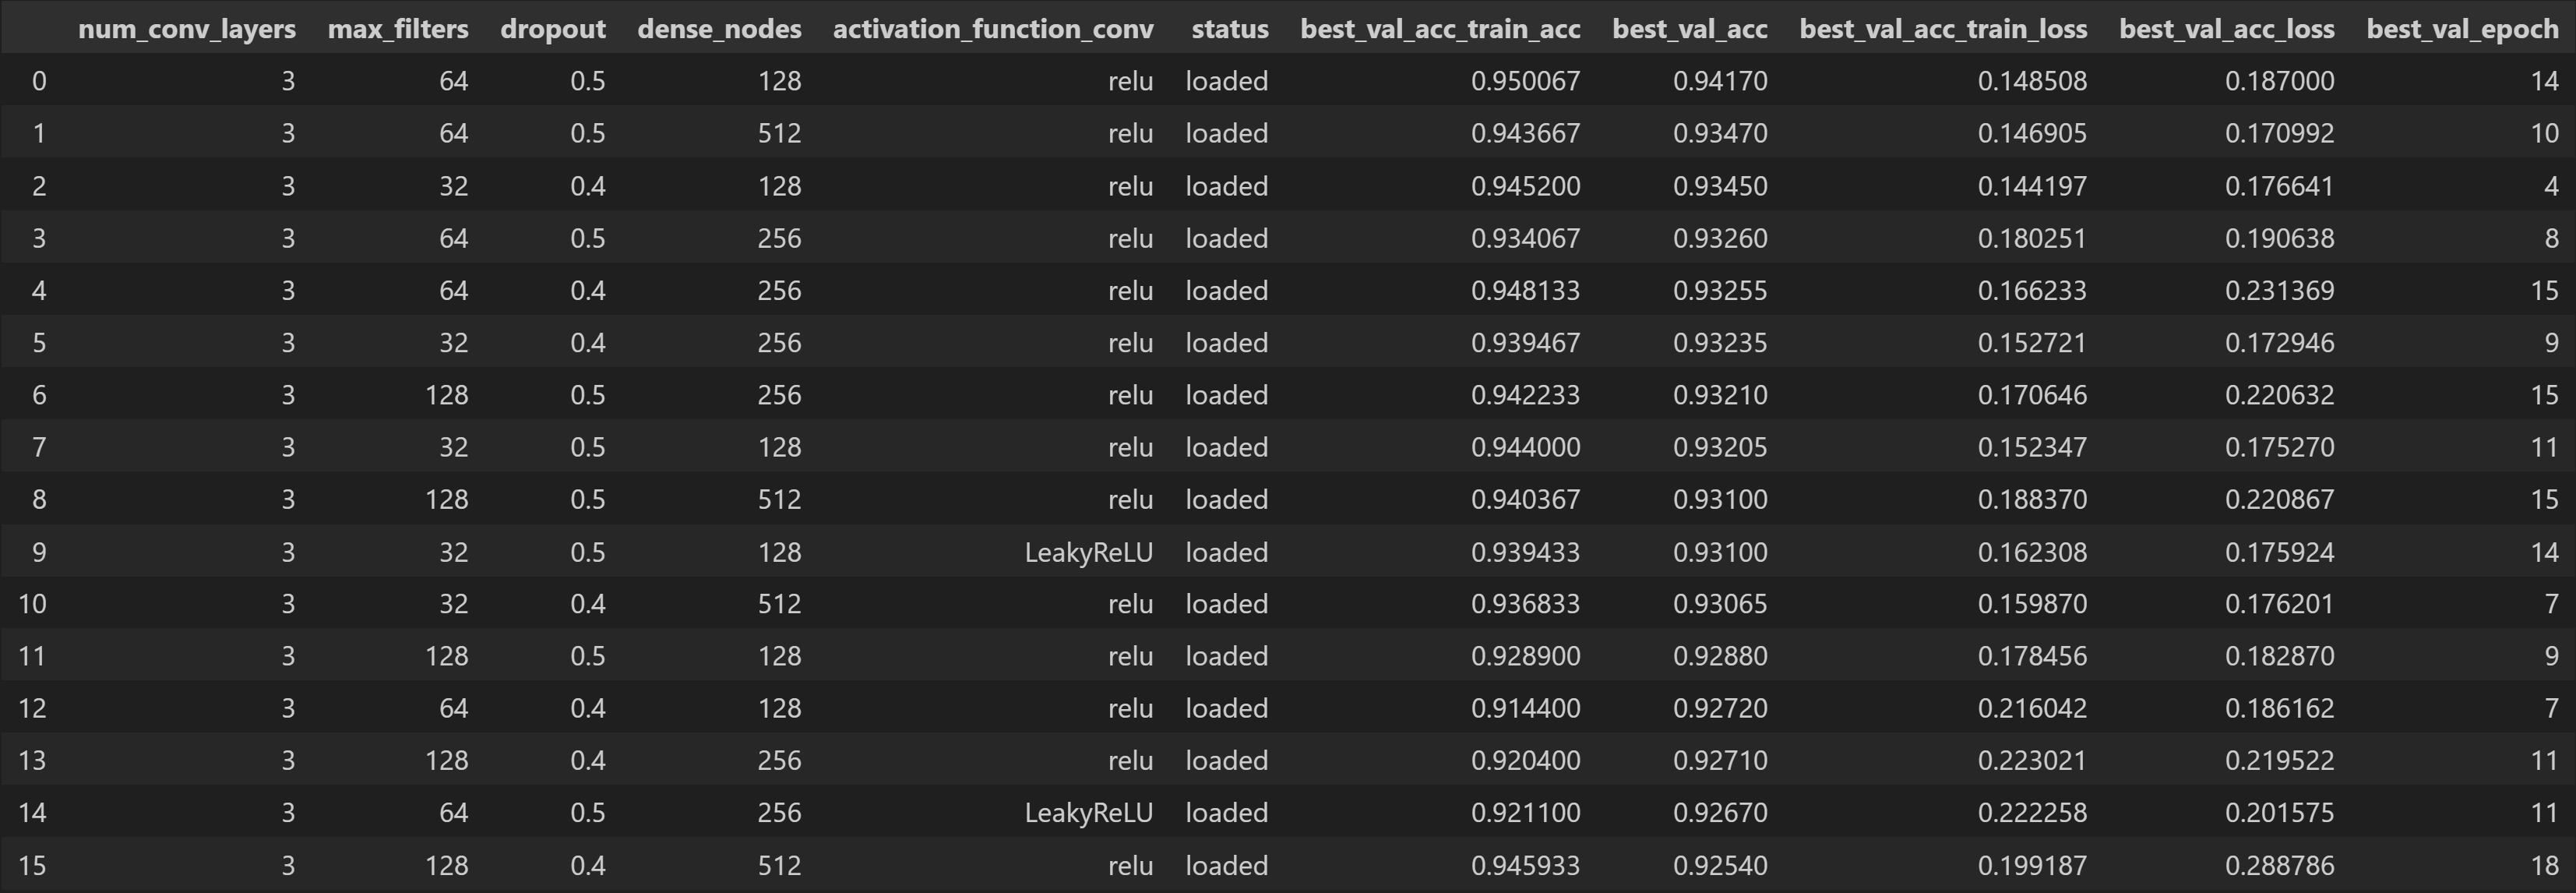
\includegraphics[width=0.6\textwidth]{images/hyperparameter_optimisation_1.png}
    \caption{The $15$ best combinations of hyperparameters for the first approach.}
    \label{fig:hyperparameter_optimisation_1}
\end{figure}


most of them performing even worse than our initial one (refer to \autoref{sec:results} for more on the hyperparameter optimisation). \\

This lead us to adapt our approach, but even with fewer layers, and without batch normalisation, the problem persisted.
As the activation function was also already changed during our hyperparameter optimisation, this didn't seem to be the cause of our problem either.
After more consideration, we arrived at three possible solutions to our problem: we could either lower the learning rate even more, train our model using cross-validation,
or try building our model on top of a model that was already trained on a large amount of images.
As the first two options would have taken a lot of training time, which already was very high, especially concerning the hyperparameter optimisation,
we decided to go with the third option.
Although unsatisfying, it was the only viable choice. \\

The pre-trained model we picked was the \texttt{VGG16}-model \cite{VGG16source}, which is a very deep convolutional model that was trained on the ImageNet dataset
and we built our model on top of it. \\

This finally yielded satisfying results, which we will discuss in the upcoming chapter.

